
%(BEGIN_QUESTION)
% Copyright 2013, Tony R. Kuphaldt, released under the Creative Commons Attribution License (v 1.0)
% This means you may do almost anything with this work of mine, so long as you give me proper credit

Examine this process trend showing the PV, SP, and Output of a loop controller:

$$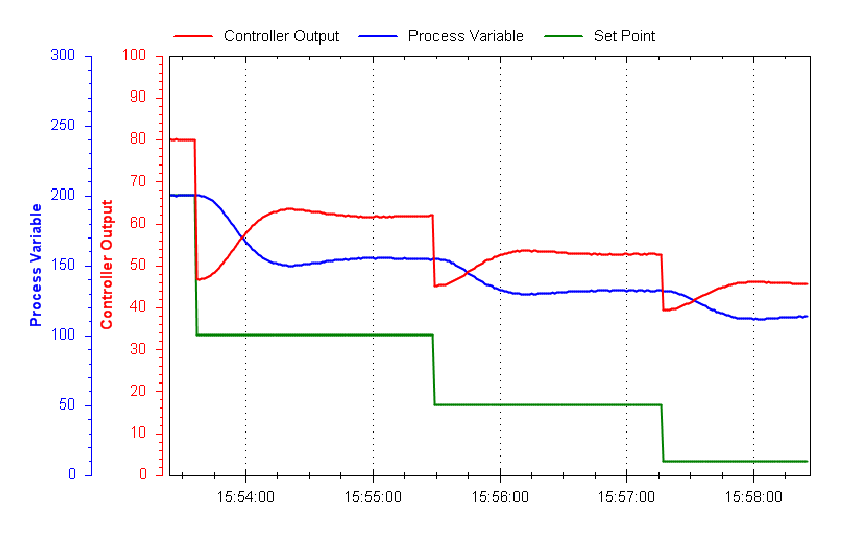
\includegraphics[width=15.5cm]{i02639x01.eps}$$

Based on what you see here, determine the following:

\begin{itemize}
\item{} Whether this is an open-loop or a closed-loop response
\item{} Whether the controller is (or needs to be) {\it direct-acting} or {\it reverse-acting}
\item{} If possible, identify any problems with the field instrumentation
\item{} If possible, identify any problems with the controller PID tuning
\item{} Qualitatively identify the kind of PID tuning we will need for robust control
\end{itemize}

\underbar{file i02639}
%(END_QUESTION)





%(BEGIN_ANSWER)

This is a {\it closed-loop test}, based on the fact the output signal responds dynamically to the changing process variable, as well as to the step-change in setpoint.

\vskip 10pt

This is a {\it reverse-acting} controller: the output steps up when the setpoint steps up (implying the output would step down if the process variable stepped up).

\vskip 10pt

There do not appear to be any field instrumentation problems revealed in this trend.  A manual-mode (open-loop) test would be more informative in that regard, but it appears as though the process is very quick to respond with no discernable dead time or other lags.

\vskip 10pt
  
The controller tuning is clearly lacking integral action.  Note the large offset between PV and SP (i.e. how the process variable never settles at the setpoint value).  This tells us the controller is configured only for proportional action, and this process needs integral!  We can also tell this from the 180$^{o}$ phase shift between PV and output during the oscillations: this is the classic response of a reverse-acting proportional-only controller.  The actual amount of gain appears to be appropriate for the loop, since the oscillations are not excessive.

\vskip 10pt

We desperately need to apply some integral action to this loop, because self-regulating loops absolutely need integral action to handle load changes and achieve new setpoint values.

%(END_ANSWER)





%(BEGIN_NOTES)


%INDEX% Process troubleshooting: diagnosing problem via trend recording

%(END_NOTES)


